\begin{comment}
\item Guest
\begin{enumerate}
  \item Registration
  \begin{itemize}
  \item She has to provide her credentials. 
  \item She has to provide her payment information.
  \item The system shall give back a password that can be used for log-in.

  \end{itemize}
  \item Log-in
  \begin{itemize}
  \item She has to provide her \gls{ID}.
  \item She has to provide her \gls{pwd}.
  %\item 

  \end{itemize}
  
  \end{enumerate}
\item User
\begin{enumerate}
  
  \item Find a car
  \begin{itemize}
  \item The system shall provide the location af all the avaible cars around the selected area.
  \item The system may know the user's location. Not necessary but useful.
  \item The system shall implement a map of the world considered.
  \end{itemize}
  
  \item Reserve a car
  \begin{itemize}
  \item The system shall kwon if a car is avaible or not.
  \item The system shall know if an user is already reserving a car.
  \item The system shall turn a car avaible or not avaible.x
  \item The system shall know the time when an user do a reservation.
  \item The system shall tag a car avaible again if a car is not picked-up within an hour from the reservation.
  \end{itemize}
  
  \item Unlock a car
  \begin{itemize}
  \item The system shall unlock a car when an user, who reaches a reserved car, tells to the system that she is nearby.
  \end{itemize}


  \item Use a car
  \begin{itemize}
  \item The system shall let each user to use only a single car at a time.
  \item The system shall start to calculate the charge as soon as the engine ignites.
  \item The system shall calculate the current cherges. The amount of money per minute is gived.
  \item The system shall notified the current charges to the user through a screen on the car.
  \end{itemize}
  
  \item Payment
  \begin{itemize}
  \item The system shall charge the user using her payment information after each utilization.
  \item The system shall start to calculate the charge as soon as the engine ignites.
  \item The system shall stop to calculate the charge as soon as the car is parked in a safe area and the user exits the car.%same moment that the car is locked
  \item The system should apply a discount of 10\% on the last ride if it detects the user took at least two other passengers onto the car.
  \item The system should apply a discount of 20\% on the last ride if the car is left with no more than 50\% of the battery empty.
  \item The system should apply a discount of 30\% on the last ride If the car is left at special parking areas where they can be recharged and the user takes care of plugging the car into the power grid.
  \item The system should charge 30\% more n the last ride if a car is left at more then 3 KM  from the nearest power grid station or with more than 80\% of the battery empty.
  \item The system shall apply a fee of 1 EUR if a car is not picked-up within an hour from the reservation.
  \end{itemize}

  \item Lock a car
  \begin{itemize}
  \item The system shall lock the car when an user has parked the car in a safe area and the user exits the car. 
  \end{itemize}

\end{enumerate}
\end{comment}


Looking at the objectives and success criteria of the project described in section 1.3, we can derive the functional requirements that PowerEnJoy have to implement. We choosed to group them by the actor involved in the function.
\begin{itemize}
  \item Guest
  \begin{enumerate}
    \item Registration
    \item Log-in
  \end{enumerate}
  \item User
  \begin{enumerate}
    \item Find a car
    \item Reserve a car
    \item Unlock a car
    \item Use a car
    \item Payment
    \item Lock a car
  \end{enumerate}
\end{itemize}

% maybe classification table (http://www.pages.drexel.edu/~sga72/docs/SRSwithUseCases.pdf)
\begin{center}
  \vspace{0.6cm}
  \begin{tabular}{|l|l|l|l|}
      \hline
      Use-case & Actor & Brief description & Goal \\\hline
      \hline
      1 & Guest & Registration & G\ref{itm:goal-registration} \\\hline
      2 & Guest & Log-in & G\ref{itm:goal-access} \\\hline
      3 & User & Reservation & G\ref{itm:goal-reservation} \\\hline
      4 & User & Use & G\ref{itm:goal-locking} \\\hline
      5 & User & Payment & G\ref{itm:goal-payment} \\\hline
  \end{tabular}
\end{center}
\begin{comment}
  \newpage
  \subsection{Sample section}
  This section is here just to provide a standard template for the system functions, before the functional requirements enumeration a brief description may be useful
  \subsubsection{Functional requirements}
  \subsubsection{Scenario 1}
  \subsubsection{Scenario 2}
  \subsubsection{Scenario n}
  \subsubsection{Use-case table}
  \subsubsection{Use-case diagram}
  \subsubsection{Activity/State-chart diagram}
  \subsubsection{Sequence diagram}
  \subsubsection{Mockups}
\end{comment}

\newpage
\subsection{Registration}
  \subsubsection{Functional Requirements}
\begin{itemize}
  \item She has to provide her credentials. 
  \item She has to provide her payment information.
  \item The system shall give back a password that can be used for log-in.
\end{itemize}
\subsubsection{Scenario 1}
Mark has been told that a new awesome car-sharing service just launched, he than decide to download the mobile application and register as a new user. After filling the sign-up module a confirmation e-mail is sent to Mark containing his new credentials.

\subsubsection{Scenario 2}
Susan was browsing the net when an advertisement caught her attention, it says: "PowerEnJoy is the new planet-friendly car sharing service! Register now and get a discount on your first ride!". She than clicks the advertisement and opens the web application: the first page is a Sign-up page and Susan fills up her personal informations and confirms. Unfortunately the informations provided are not complete and the system signals an error, she notices that the driving licence's informations are missing and compiles the remaining part of the module before submitting it and receiving a confirmation e-mail.

\subsubsection{Use-case table}
\begin{center}
  \begin{tabular}{ l | p{12cm} }
    \hline
    Actors & Guest\\ \hline
    Goal & G\ref{itm:goal-registration}\\ \hline
    Entry conditions & 
\begin{itemize}
\item The Guest has to have internet access.
\item The Guest entres the Sign-up page in the browser/ mobile application. 
\end{itemize} \\ \hline
    Flow of events &
\begin{itemize} % todo: shrink items
\item The Guest is shown a form to fill with her personal e-mail, name, surname, tax code and phone number. %da scegliere se l'ID viene scelto dal system o dal Guest 
\item The Guest fills the form and confirm her provided information.
\item The Guest is shown a form to fill with her drive license's information.
\item The Guest fills the form and confirm her provided information.
\item The Guest is shown a form to fill with her payment information.
\item The Guest fills the form and confirm her provided information.
\item The system sends a confirmation e-mail to the Guest's personal e-mail with an activation link.
\item The Guest clicks the link in the system's e-mail.
\item The system allocates the User in the database.
\item The system sends an e-mail to the User's e-mail with her personal \gls{pwd}.
\item The system loads the User's homepage.
\end{itemize} \\ \hline
  	Exit conditions & The Guest is registered to PowerEnJoy and became an User. Now the User is in her homepage. \\ \hline
	Exceptions & 
\begin{itemize}
\item The Guest provides an e-mail or a phone number or a tax code already used (in this case the system signals an error).
\item The Guest does not fill one or more fields in a form (in this cases the system does not allow to proceed and signals an InformationLack).
\item The Guest provided wrong payment information (in this case the system signals an error).
\item The Guest provided wrong drive license information (in this case the system signals an error).
\item The system is not able to complete the operation due to some internal issues or connection broken (the system signals a CennectionToSystemFail).%volendo si possono modificare i nomi delle eccezzioni.
\end{itemize} \\ \hline
  \end{tabular}
\end{center}


\newpage
\subsection{Log-in}
  \subsubsection{Functional Requirements}
\begin{itemize}
  \item The user must provide a valid ID.
  \item The user must provide a valid password.
\end{itemize}

\subsubsection{Scenario 1}
Susan has just registered to PowerEnJoy and loads the home page in order to login, she then enters her credentials and submit the form. The credential are checked and Susan is redirected to the web application as a logged user.

\subsubsection{Scenario 2}
Mark is a typical PowerEnJoy user, he got used to the credentials form submission and types his password quickly. The password is not recognized by the system and Mark is asked to check his credentials. He then types more accurately and finally gets redirected to the web application. % todo: maybe forgot password

\subsubsection{Scenario 3}
A guest confused the login form with the registration one and after submiting the form is told that such user is not registered to the PowerEnJoy service. She then clicks on "Register to PowerEnJoy" and follows the registration procedure.


\subsubsection{Mockups}
\begin{figure}[!ht]
  \centering
  \vspace{0.2cm}
  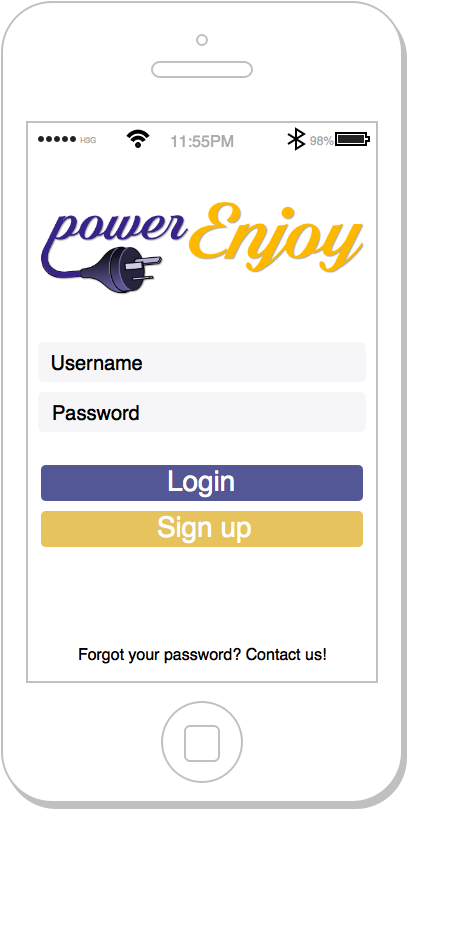
\includegraphics[width=0.25\textwidth]{/RASD/System_Functions/login_mockup}\\
  \vspace{0.4cm}
  %\caption{Mockup for the login mobile page} 
  \label{fig:login_mockup} 
\end{figure}
% maybe home page mockup here 


\subsubsection{Use-case table}
\begin{center}
  \begin{tabular}{ l | p{10cm} }
    \hline
    Actors & Guest\\ \hline
    Goal & G\ref{itm:goal-session}\\ \hline
    Entry conditions & The Guest is registered to PowerEnJoy and browse to the Log-in page in the web/mobile application. \\ \hline
    Flow of events &
\begin{itemize}
\item The Guest insert her \gls{ID} and \gls{pwd}.
\item The Guest clicks the Log-in button.
\item The system loads the User's homepage.
\end{itemize} \\ \hline
    Exit conditions & The User is in the PowerEnJoy homepage. \\ \hline
  Exceptions & 
\begin{itemize}
\item The Guest provides wrong username-password pair (the system signals a LoginError).
\item The Guest doesn't fill one of the fields (the systems signals an InformationLack).
\item The system is not able to complete the operation due to some internal issues or connection broken (the system signals a ConnectionFailure).
\end{itemize} \\ \hline
  \end{tabular}
\end{center}


\subsubsection{Sequence diagram}
\begin{figure}[!ht]
  \centering
  \vspace{0.1cm}
  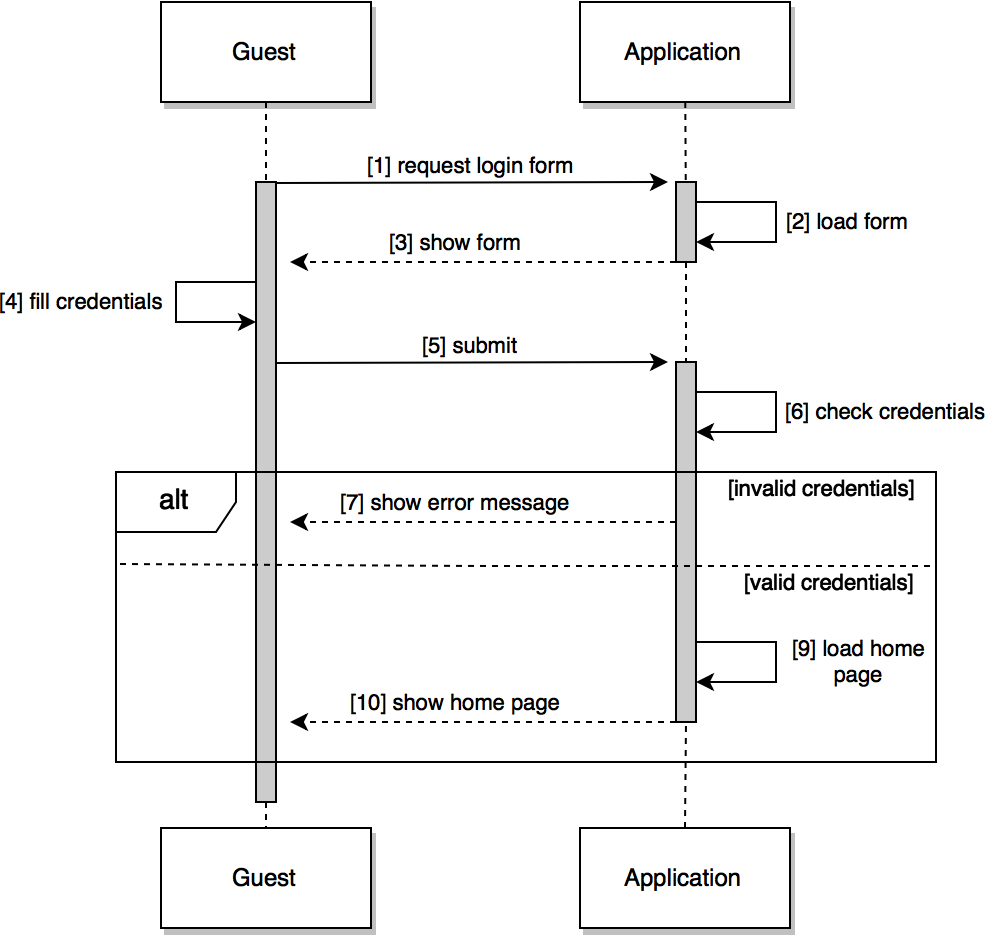
\includegraphics[width=0.6\textwidth]{/RASD/System_Functions/login_sequence}\\
  \vspace{0.1cm}
  %\caption{Sequence diagram for the login procedure} 
  \label{fig:login_sequence} 
\end{figure}



\newpage
\subsection{Manage account}
  \subsubsection{Functional Requirements}
\begin{itemize}
  \item The system must store all the account information.
  \item The user must be able to modify the password.
  \item The system must update any changed information.
  \item he system shall check that all the informations are valid.
\end{itemize}

\subsubsection{Scenario 1}
After five months that Susan is using PowerEnJoyshe she has decided that is better to change her \gls{pwd}. So she open her manage profile page and change it. Then she save the changes and the system upload Susan's information. Then for the future acesses Susan will use her new \gls{pwd}.

\subsubsection{Scenario 2}
Mark is a typical PowerEnJoy user. Unfortunatly his credic card is expired and so he has to change it. He was using that credit card also for pay his PowerEnJoy's charges. So as soon as he has his new credit card he decides to upload his payment information on PowerEnJoy. He accesses his manage profile page and changed the payment information. Since that moment PowerEnJoy is going to charge Mark on his new credit card.



\subsubsection{Mockups}
\begin{figure}[!ht]
  \centering
  \vspace{0.2cm}
  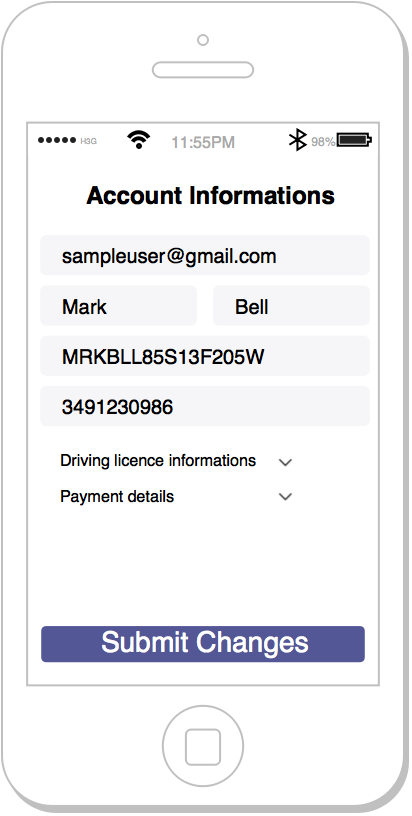
\includegraphics[width=0.25\textwidth]{/RASD/System_Functions/manage_account_mockup}\\
  \vspace{0.4cm}
  %\caption{Mockup for the account management mobile page} 
  \label{fig:manage_account_mockup} 
\end{figure}


\subsubsection{Use-case table}
\begin{center}
  \begin{tabular}{ l | p{10cm} }
    \hline
    Actors & User\\ \hline
    Goal & G\ref{itm:goal-account}\\ \hline
    Entry conditions & The User is logged into the system and she is viewing her profile page.   
    \\ \hline
    Flow of events &
      \begin{itemize}
        \item The User select the "Modify profile" option.
        \item The User modifies one or more information.
        \item The User submit the modifications.
        \item The system checks the modifications and upload them.
      \end{itemize} 
      \\ \hline
    Exit conditions & The User's profile is modified. \\ \hline
  Exceptions & 
\begin{itemize}
\item The User provides empty or invalid values as modifications (the system signals an error).
\item The User doesn't submit the modifications (the system aborts the request).
\item The system is not able to complete the operation due to some internal issues or connection broken (the system signals a ConnectionFailure).
\end{itemize} \\ \hline
  \end{tabular}
\end{center}


\subsubsection{Sequence diagram}
\begin{figure}[!ht]
  \centering
  \vspace{0.1cm}
  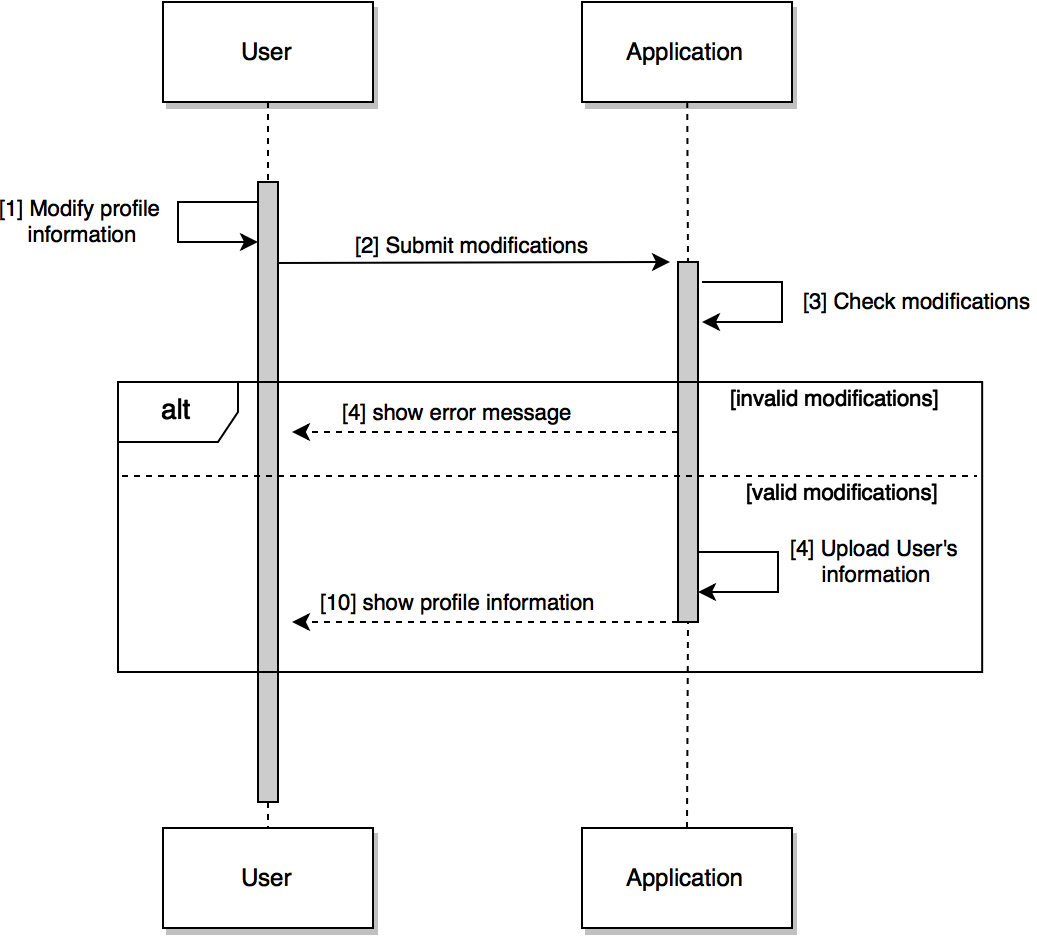
\includegraphics[width=0.6\textwidth]{/RASD/System_Functions/manage_account_sequence}\\
  \vspace{0.1cm}
  %\caption{Sequence diagram for the account management procedure} 
  \label{fig:manage_account_sequence} 
\end{figure}



\newpage
\subsection{Create Reservation}
  \subsubsection{Functional Requirements}
\begin{itemize}
  \item The system shall kwon if a car is avaible or not.
  \item The system shall know if an user is already reserving a car.
  \item The system shall turn a car avaible or not avaible.
  \item The system shall know the time when an user do a reservation.
  \item The system shall tag a car avaible again if a car is not picked-up within an hour from the reservation.
\end{itemize}

\subsubsection{Scenario 1}
Mark needs to go to the city center in the late evening and decides to use a PowerEnJoy's car. Just before having a quick lunch in a near restaurant he browses the application and reserves car near him to make sure that it will still be available when he'll be back.
Unexpectedly Morgan, a friend of Mark, is lunching in the same restaurant and when they see each other they start chatting about everything and anything. When they stop talking Mark notices an e-mail from PowerEnJoy: it's about his reservation that has expired. His bank has also notified him that a fee of 1€ was applied by PowerEnJoy.


\subsubsection{Scenario 2}
Susan is a typical PowerEnJoy user, she was walking through a street when a friend texts her to hang out. Fortunately she saw a PowerEnJoy's car on the other side of the street. She reached the car and checked online: that's not available. Someone had probably already reserved it. But on the app she noticed that there were two avable car 5 minutes walk from her position. Than she reserved one of that two cars and easily reached it, thanks to the accurate location service provided by the system. 


\subsubsection{Mockups}
\begin{figure}[!ht]
  \centering
  \vspace{0.1cm}
  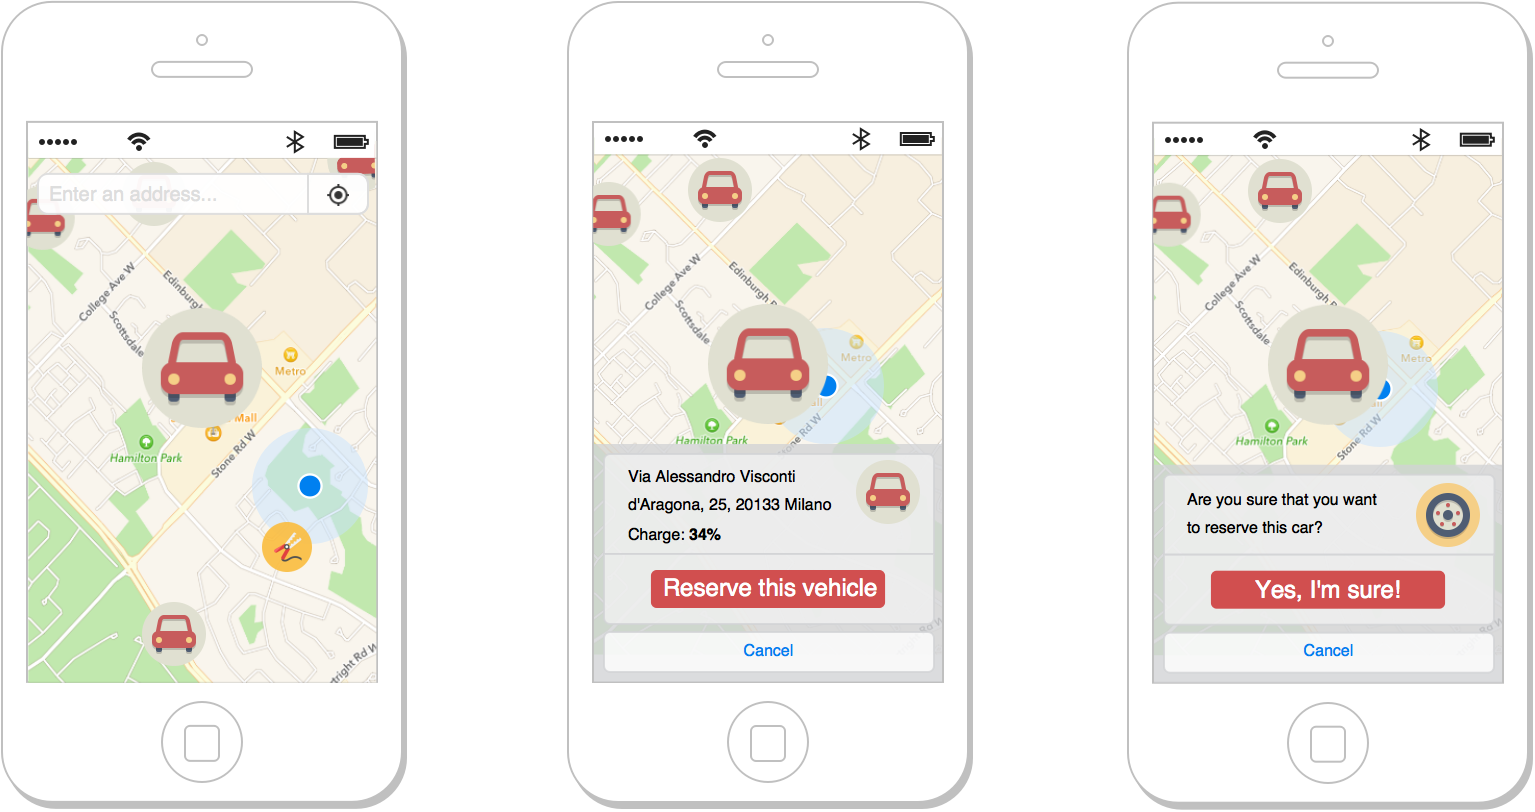
\includegraphics[width=1\textwidth]{/RASD/System_Functions/create_reservation_mockup}\\
  \vspace{0.4cm}
  %\caption{Mockup for the login mobile page} 
  \label{fig:create_reservation_mockup} 
\end{figure}
% maybe home page mockup here 


\subsubsection{Use-case table}
\begin{center}
  \begin{tabular}{ l | p{10cm} }
    \hline
    Actors & Guest\\ \hline
    Goal & G\ref{itm:goal-reservation}\\ \hline
    Entry conditions & \begin{itemize}
			\item The User is in his homepage and want to reserve a car.
			\item PowerEnJoy has available cars.
			\item The User is not already reserving a car.
\end{itemize}  \\ \hline
    Flow of events &
\begin{itemize}
%\item The User select the "Find a car" option.
\item The User has three ways for finding a car:
\begin{itemize}
			\item browse the map.
			\item use her location.
			\item enters an address.
\end{itemize}
%\item The system loads a map of the selected area and the avaible cars' locations near there .
\item The User selects the car that want to reserve.
\item the system displays the car's information.%Maybe to add to the mockup
%\item The User presses the "Yes,I'm sure" button for confirm the reservation.
\item The system turn the car "reserved".% and start the reservation timer.
\item The system notified the User.
\end{itemize} \\ \hline
    Exit conditions &
\begin{itemize}
	\item A car is set as "reserved".
	\item The car is reserved for up one hour. After that the reservation expires and the User has to pay a fee of 1€.
\end{itemize}  \\ \hline
  Exceptions & 
%\begin{itemize}
%\item The User has already reserved a car.

%\item 
The system is not able to complete the operation due to some internal issues or connection broken (the system signals a ConnectionFailure).%volendo si possono modificare i nomi delle eccezzioni.
%\end{itemize} 
\\ \hline
  \end{tabular}
\end{center}


\subsubsection{Sequence diagram}
\begin{figure}[!ht]
  \centering
  \vspace{0.2cm}
  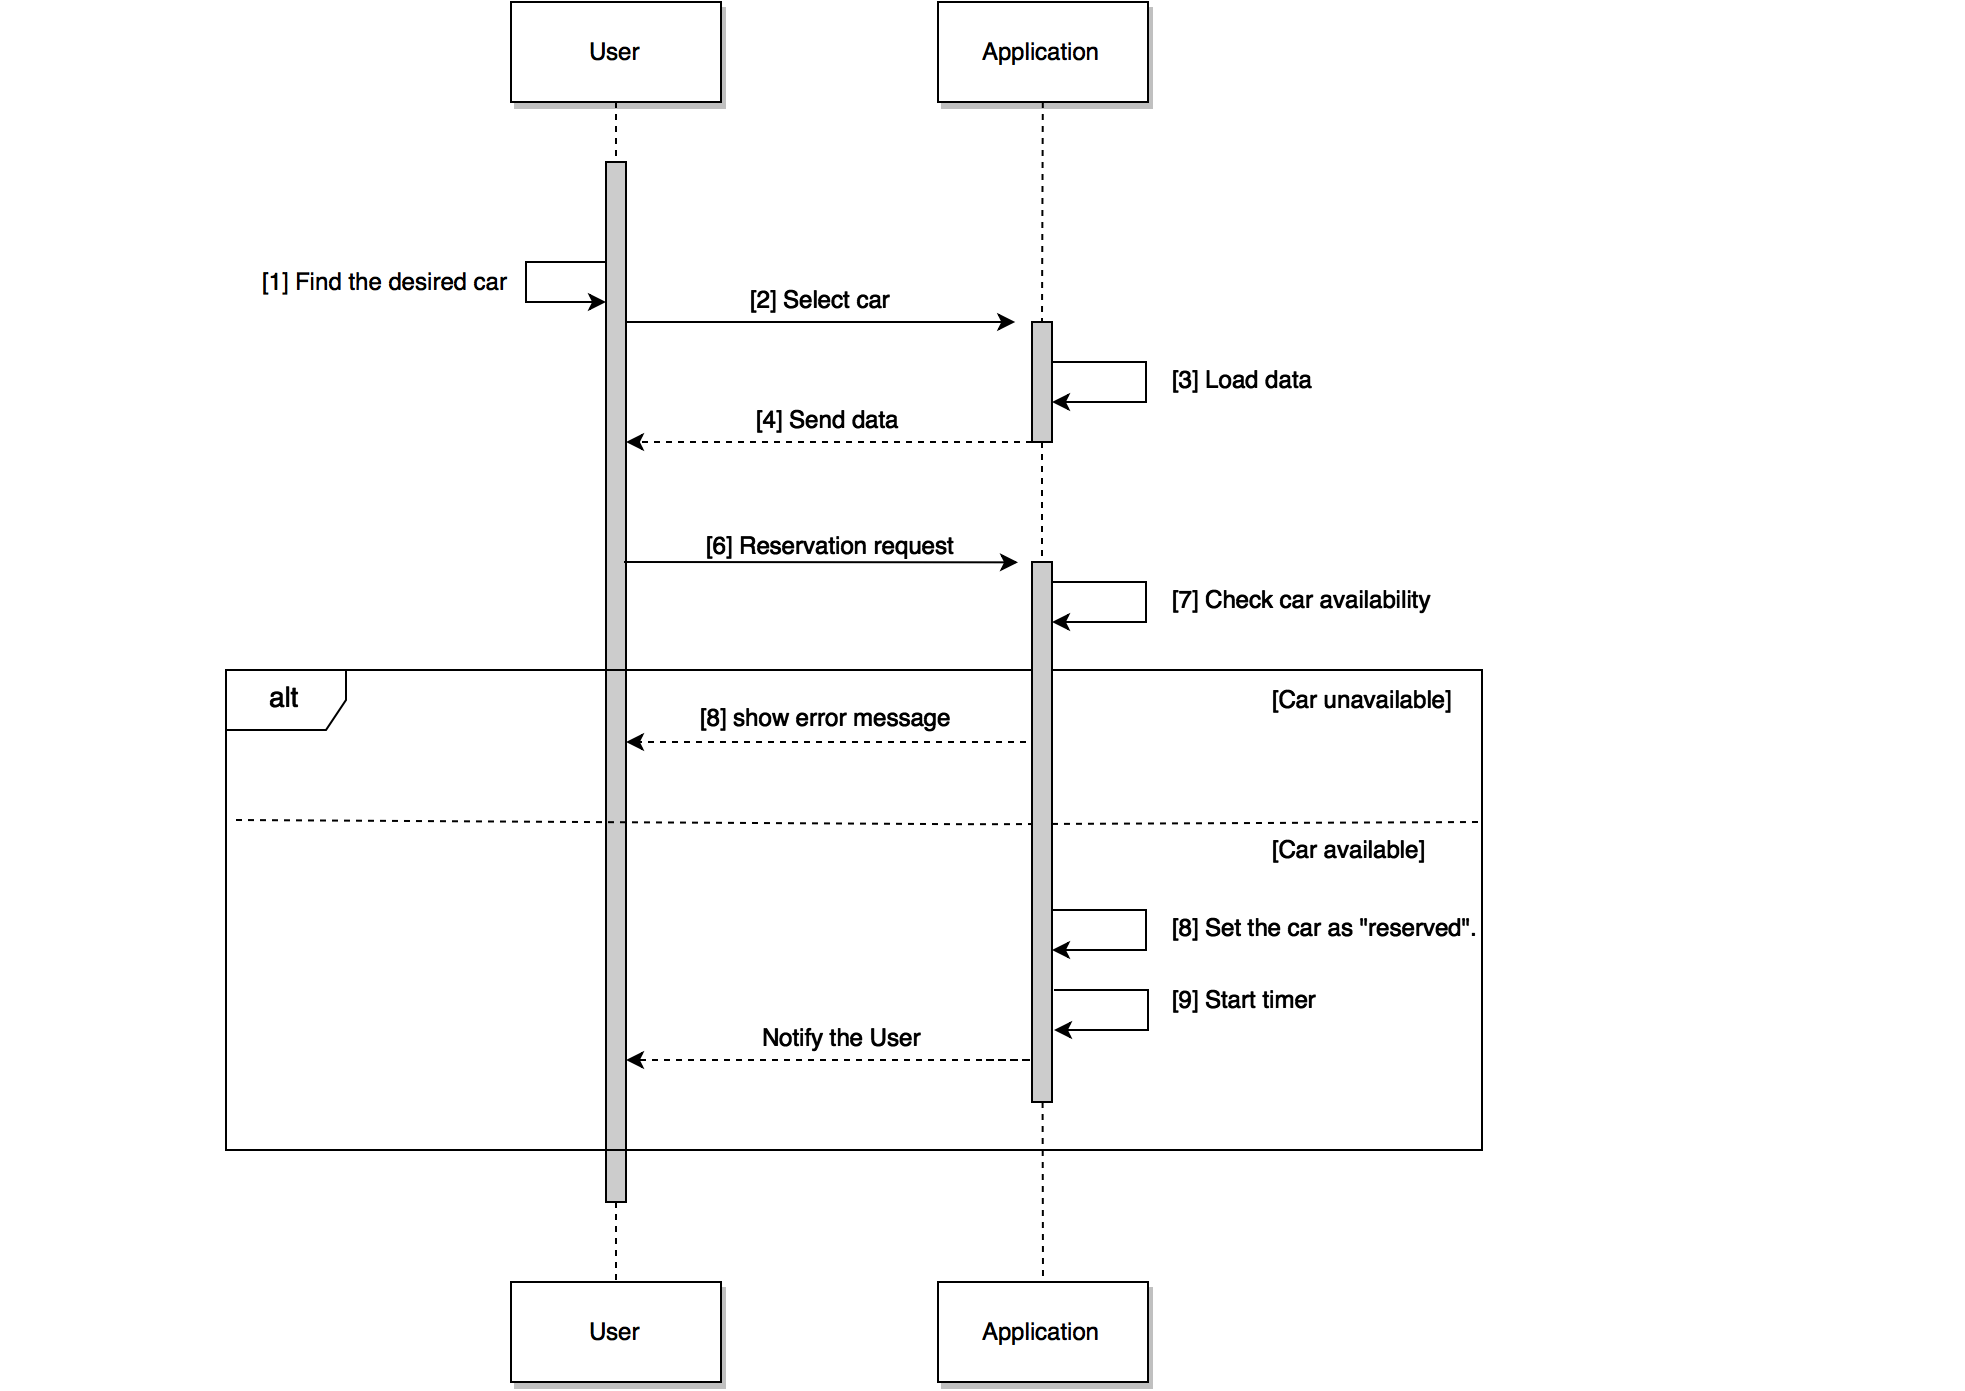
\includegraphics[width=1.2\textwidth]{/RASD/System_Functions/reservation_sequence}\\
  \vspace{0.1cm}
  %\caption{Sequence diagram for the login procedure} 
  \label{fig:reservation_sequence} 
\end{figure}



\newpage
\subsection{Expiration of the reservation}
  \input{contents/Requirements_Specification/System_Functions/Expiration_of_the_reservation}
  
%\newpage
%\subsection{Menage Account}
%  \subsubsection{Functional Requirements}
\begin{itemize}
  \item The system must store all the account information.
  \item The user must be able to modify the password.
  \item The system must update any changed information.
  \item he system shall check that all the informations are valid.
\end{itemize}

\subsubsection{Scenario 1}
After five months that Susan is using PowerEnJoyshe she has decided that is better to change her \gls{pwd}. So she open her manage profile page and change it. Then she save the changes and the system upload Susan's information. Then for the future acesses Susan will use her new \gls{pwd}.

\subsubsection{Scenario 2}
Mark is a typical PowerEnJoy user. Unfortunatly his credic card is expired and so he has to change it. He was using that credit card also for pay his PowerEnJoy's charges. So as soon as he has his new credit card he decides to upload his payment information on PowerEnJoy. He accesses his manage profile page and changed the payment information. Since that moment PowerEnJoy is going to charge Mark on his new credit card.



\subsubsection{Mockups}
\begin{figure}[!ht]
  \centering
  \vspace{0.2cm}
  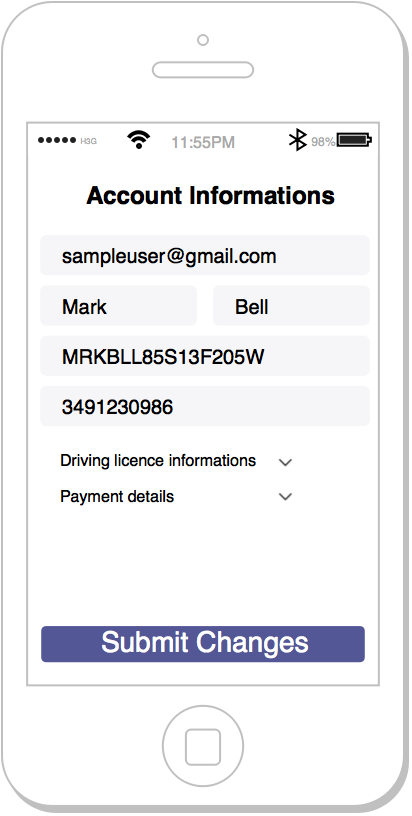
\includegraphics[width=0.25\textwidth]{/RASD/System_Functions/manage_account_mockup}\\
  \vspace{0.4cm}
  %\caption{Mockup for the account management mobile page} 
  \label{fig:manage_account_mockup} 
\end{figure}


\subsubsection{Use-case table}
\begin{center}
  \begin{tabular}{ l | p{10cm} }
    \hline
    Actors & User\\ \hline
    Goal & G\ref{itm:goal-account}\\ \hline
    Entry conditions & The User is logged into the system and she is viewing her profile page.   
    \\ \hline
    Flow of events &
      \begin{itemize}
        \item The User select the "Modify profile" option.
        \item The User modifies one or more information.
        \item The User submit the modifications.
        \item The system checks the modifications and upload them.
      \end{itemize} 
      \\ \hline
    Exit conditions & The User's profile is modified. \\ \hline
  Exceptions & 
\begin{itemize}
\item The User provides empty or invalid values as modifications (the system signals an error).
\item The User doesn't submit the modifications (the system aborts the request).
\item The system is not able to complete the operation due to some internal issues or connection broken (the system signals a ConnectionFailure).
\end{itemize} \\ \hline
  \end{tabular}
\end{center}


\subsubsection{Sequence diagram}
\begin{figure}[!ht]
  \centering
  \vspace{0.1cm}
  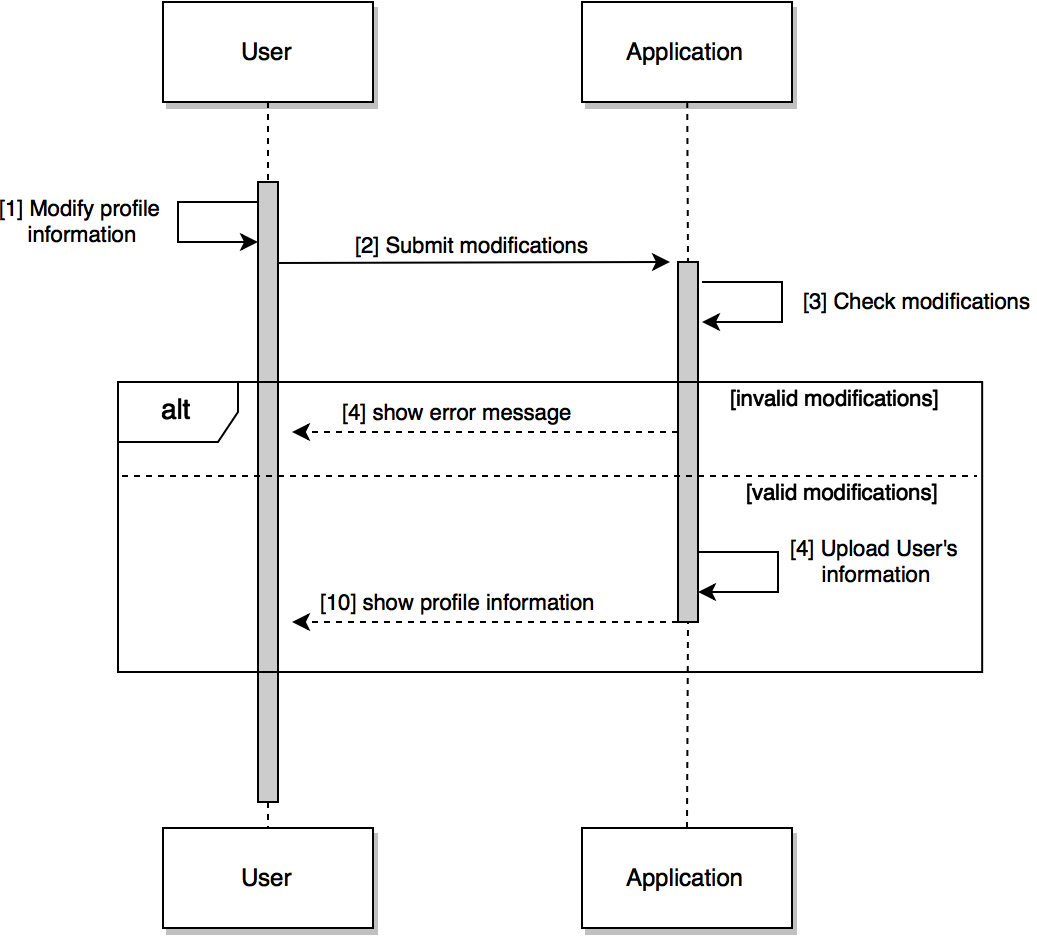
\includegraphics[width=0.6\textwidth]{/RASD/System_Functions/manage_account_sequence}\\
  \vspace{0.1cm}
  %\caption{Sequence diagram for the account management procedure} 
  \label{fig:manage_account_sequence} 
\end{figure}


  
\newpage
\subsection{Delete Reservation}
  \subsubsection{Functional Requirements}
\begin{itemize}
  \item The system must tag a car avaible again if a related reservation is deleted.
  \item The system must not apply any charge if the reservation is deleted before expiration.
\end{itemize}


\subsubsection{Scenario 1}
Michael is in a hurry because he has a meeting downtown in 20 minutes, he is really late and after locating a PowerEnJoy car he submits a reservation. He is about to unlock the car when he hears someone calling his name, a collegue recognized him and stopped to offer him a ride. Michael accepts but he immediately cancels his reservation in order to avoid the expiration fine and allow other users to take advantage of the service. The system processed his request and now the car is available again. 


\subsubsection{Mockups}
\begin{figure}[!ht]
  \centering
  \vspace{0.2cm}
  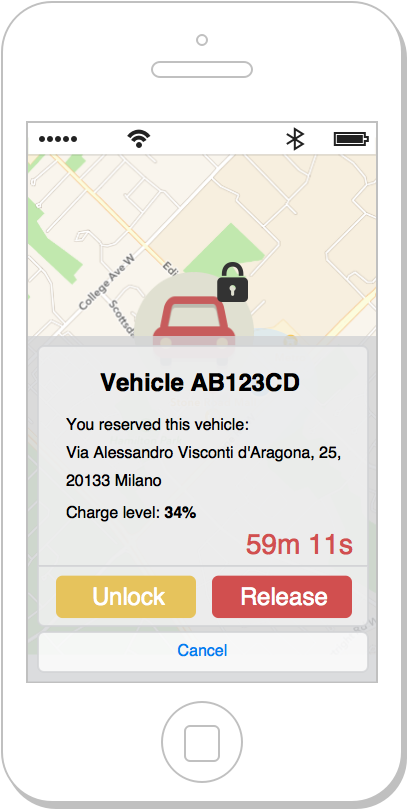
\includegraphics[width=0.25\textwidth]{/RASD/System_Functions/delete_reservation_mockup}\\
  \vspace{0.4cm}
  %\caption{Mockup for the reservation deletion mobile page} 
  \label{fig:delete_reservation} 
\end{figure}
% maybe home page mockup here 


\subsubsection{Use-case table}
\begin{center}
  \begin{tabular}{ l | p{10cm} }
    \hline
    Actors & User\\ \hline
    Goal & G\ref{itm:goal-reservation}\\ \hline
    Entry conditions & The User has previously reserved a vehicle and wants to delete the reservation
     \\ \hline
    Flow of events &
    \begin{itemize} 
      \item The User opens the application 
      \item The Users visualizes in his home page the active reservation
      \item The User clicks "Delete" in order to release his reservation
      \item The system processes his request and updates the car status
      \item The system loads the User's homepage.
    \end{itemize} \\ \hline
    Exit conditions & The User is in his homepage but his last reservation has been deleted and the vehicle is free again \\ \hline
  	Exceptions & 
    \begin{itemize}
      \item The reservation is already expired (the system signals an error).
      \item The system is not able to complete the operation due to some internal issues or connection broken (the system signals a ConnectionFailure).
    \end{itemize} \\ \hline
  \end{tabular}
\end{center}


\subsubsection{Sequence diagram}
\begin{figure}[!ht]
  \centering
  \vspace{0.2cm}
  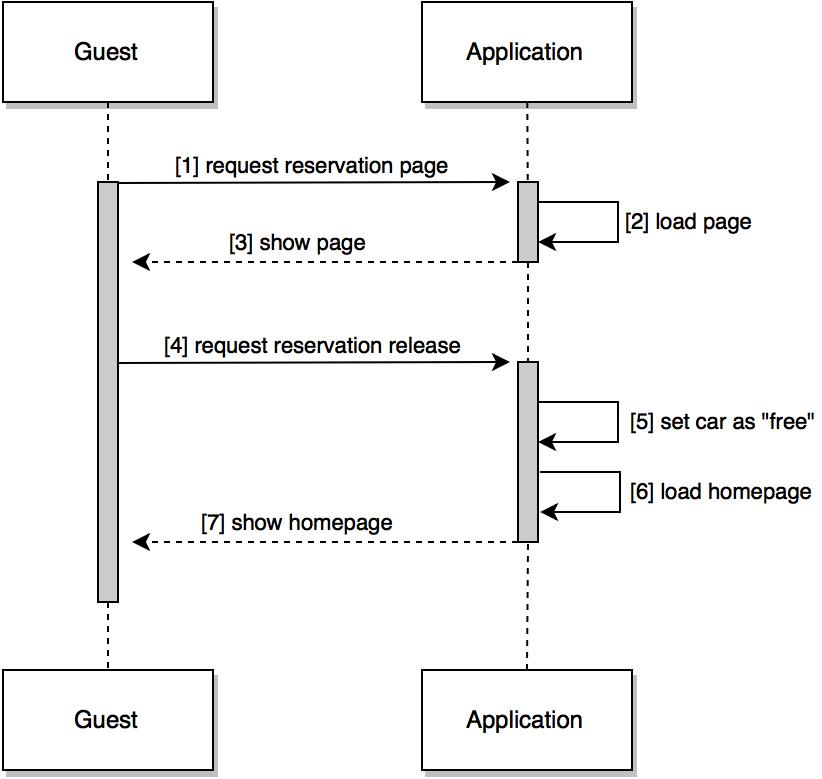
\includegraphics[width=0.8\textwidth]{/RASD/System_Functions/delete_reservation_sequence}\\
  \vspace{0.4cm}
  %\caption{Sequence diagram for the reservation release procedure} 
  \label{fig:delete_reservation_sequence} 
\end{figure}


\newpage
\subsection{Charge Ride}
   \input{contents/Requirements_Specification/System_Functions/Charge_Ride}

\newpage
\subsection{Discounts \& Fees}
   \subsubsection{Functional Requirements}
\begin{itemize}
  \item The system shall kwon if a car is avaible or not.
  \item The system shall know if an user is already reserving a car.
  \item The system shall turn a car avaible or not avaible.
  \item The system shall know the time when an user do a reservation.
  \item The system shall tag a car avaible again if a car is not picked-up within an hour from the reservation.
\end{itemize}

\subsubsection{Scenario 1}
Mark needs to go to the city center in the late evening and decides to use a PowerEnJoy's car. Just before having a quick lunch in a near restaurant he browses the application and reserves car near him to make sure that it will still be available when he'll be back.
Unexpectedly Morgan, a friend of Mark, is lunching in the same restaurant and when they see each other they start chatting about everything and anything. When they stop talking Mark notices an e-mail from PowerEnJoy: it's about his reservation that has expired. His bank has also notified him that a fee of 1€ was applied by PowerEnJoy.


\subsubsection{Scenario 2}
Susan is a typical PowerEnJoy user, she was walking through a street when a friend texts her to hang out. Fortunately she saw a PowerEnJoy's car on the other side of the street. She reached the car and checked online: that's not available. Someone had probably already reserved it. But on the app she noticed that there were two avable car 5 minutes walk from her position. Than she reserved one of that two cars and easily reached it, thanks to the accurate location service provided by the system. 


\subsubsection{Mockups}
\begin{figure}[!ht]
  \centering
  \vspace{0.1cm}
  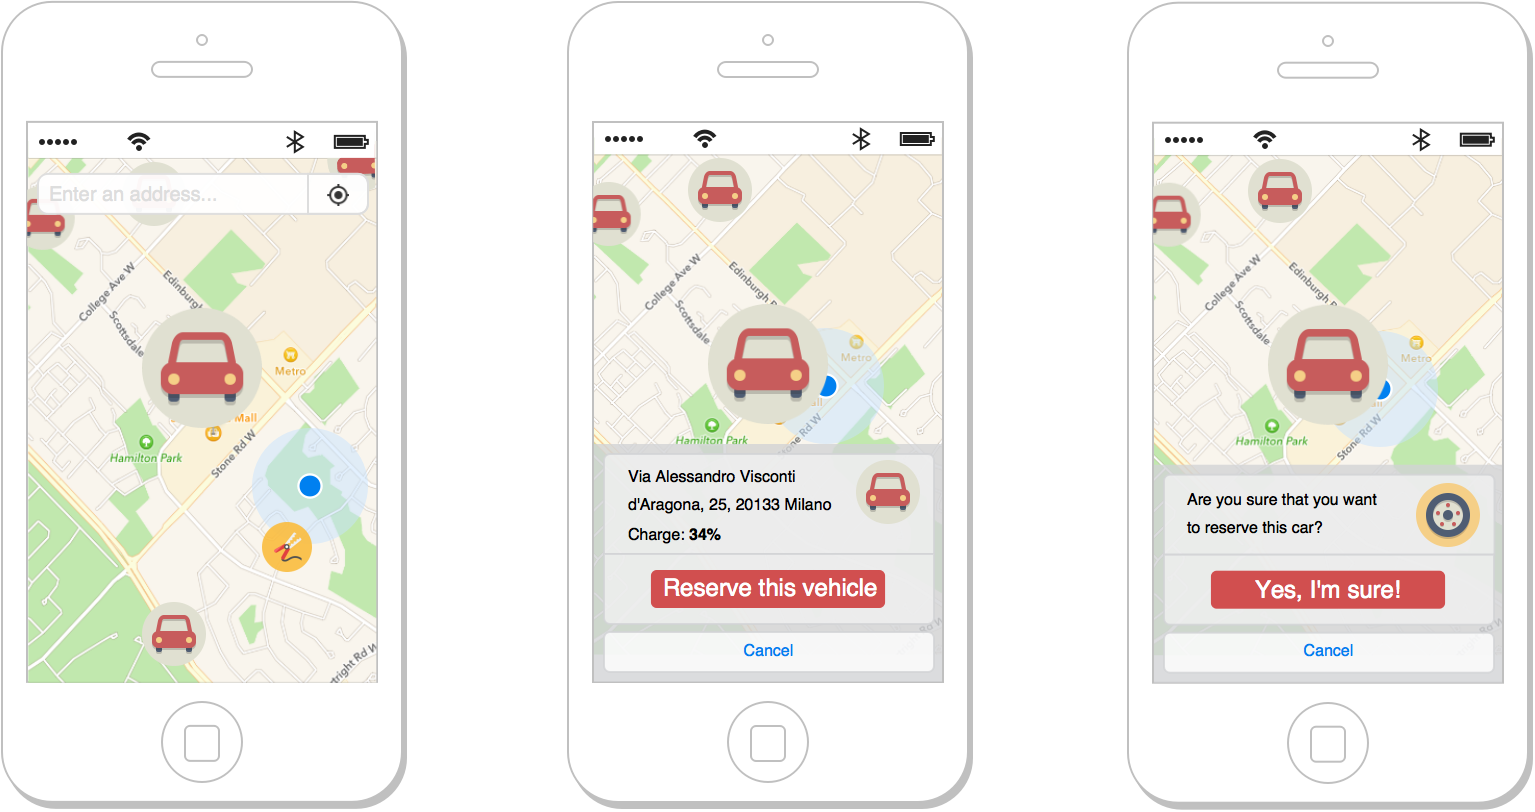
\includegraphics[width=1\textwidth]{/RASD/System_Functions/create_reservation_mockup}\\
  \vspace{0.4cm}
  %\caption{Mockup for the login mobile page} 
  \label{fig:create_reservation_mockup} 
\end{figure}
% maybe home page mockup here 


\subsubsection{Use-case table}
\begin{center}
  \begin{tabular}{ l | p{10cm} }
    \hline
    Actors & Guest\\ \hline
    Goal & G\ref{itm:goal-reservation}\\ \hline
    Entry conditions & \begin{itemize}
			\item The User is in his homepage and want to reserve a car.
			\item PowerEnJoy has available cars.
			\item The User is not already reserving a car.
\end{itemize}  \\ \hline
    Flow of events &
\begin{itemize}
%\item The User select the "Find a car" option.
\item The User has three ways for finding a car:
\begin{itemize}
			\item browse the map.
			\item use her location.
			\item enters an address.
\end{itemize}
%\item The system loads a map of the selected area and the avaible cars' locations near there .
\item The User selects the car that want to reserve.
\item the system displays the car's information.%Maybe to add to the mockup
%\item The User presses the "Yes,I'm sure" button for confirm the reservation.
\item The system turn the car "reserved".% and start the reservation timer.
\item The system notified the User.
\end{itemize} \\ \hline
    Exit conditions &
\begin{itemize}
	\item A car is set as "reserved".
	\item The car is reserved for up one hour. After that the reservation expires and the User has to pay a fee of 1€.
\end{itemize}  \\ \hline
  Exceptions & 
%\begin{itemize}
%\item The User has already reserved a car.

%\item 
The system is not able to complete the operation due to some internal issues or connection broken (the system signals a ConnectionFailure).%volendo si possono modificare i nomi delle eccezzioni.
%\end{itemize} 
\\ \hline
  \end{tabular}
\end{center}


\subsubsection{Sequence diagram}
\begin{figure}[!ht]
  \centering
  \vspace{0.2cm}
  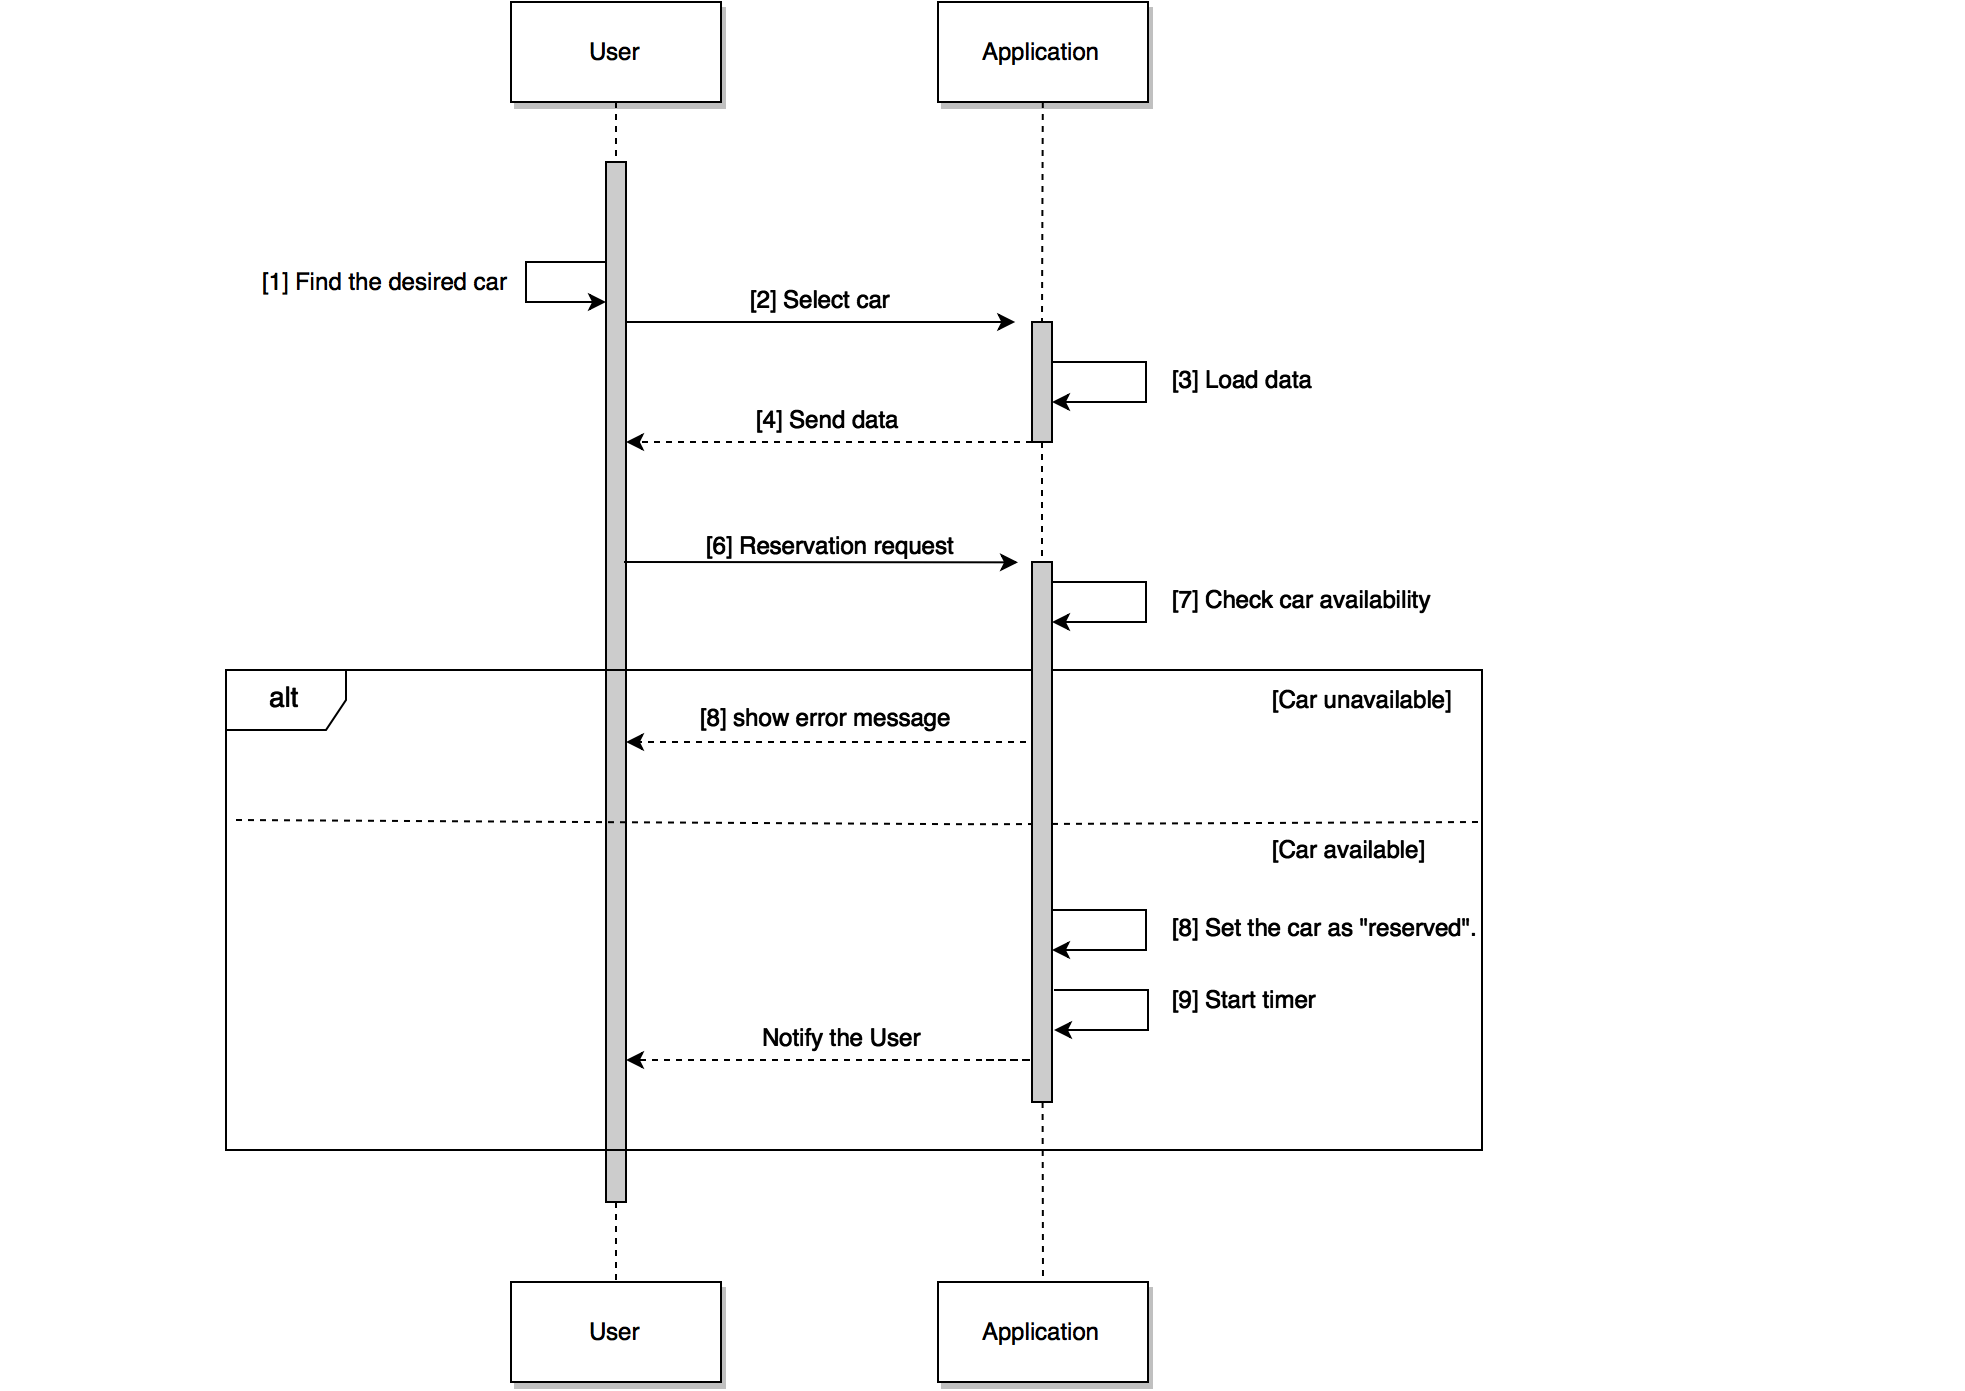
\includegraphics[width=1.2\textwidth]{/RASD/System_Functions/reservation_sequence}\\
  \vspace{0.1cm}
  %\caption{Sequence diagram for the login procedure} 
  \label{fig:reservation_sequence} 
\end{figure}




